\documentclass[10pt, uplatex, dvipdfmx]{jsarticle}
\usepackage{../mypackage}

\graphicspath{{../pictures}}

\setcounter{section}{7}

\begin{document}

\section{$2$ 重積分の計算(累次積分)}

\subsection{縦線集合・横線集合上の2重積分}

2重積分の計算は次の定理を使うのが一般的である.この定理の証明はおまけとして\ref{subsec:pf-iterated2}節で述べる.

\begin{theorem}\label{thm:iterated2}
  $f(x,y)$ を有界閉領域 $D$ 上連続な $2$ 変数関数とする.
  \begin{enumerate}[(1)]
    \setlength{\itemsep}{.1in}

  \item 実数 $a,b$ と閉区間 $[a,b]$ 上 $\varphi_1(x) \leqq
    \varphi_2(x)$ かつ連続な関数 $\varphi_1, \varphi_2$ によって $D$ が
    \[
      D=\Set{(x,y) | a \leqq x \leqq b, \, \varphi_1(x) \leqq y \leqq \varphi_2(x)}
    \]
    と表せるとき,$f(x,y)$ は $D$ 上重積分可能で以下が成り立つ.
    \[
      \iint_{D} f(x,y) \ dx dy = \int_{a}^{b} \left( \int_{\varphi_1(x)}^{\varphi_2(x)} f(x,y)\ dy\right) dx 
    \]

  \item 実数 $c,d$ と閉区間 $[c,d]$ 上 $\psi_1(y) \leqq
    \psi_2(y)$ かつ連続な関数 $\psi_1, \psi_2$ によって $D$ が
    \[
      D=\Set{(x,y) | c \leqq y \leqq d, \, \psi_1(y) \leqq x \leqq  \psi_2(y)}
    \]
    と表せるとき,$f(x,y)$ は $D$ 上重積分可能で以下が成り立つ.
    \[
      \iint_{D} f(x,y) \ dx dy = \int_{c}^{d} \left( \int_{\psi_1(y)}^{\psi_2(y)} f(x,y) \ dx \right) dy
    \]\\
  \end{enumerate}
  
\end{theorem}



定理\ref{thm:iterated2}(1)の $D$ を\textbf{縦線集合}(左下図)といい,
(2)の $D$ を\textbf{横線集合}(右下図)という.
\begin{figure}[h]
  \centering
  \begin{tabular}{c}
    \begin{minipage}{0.45\linewidth}
      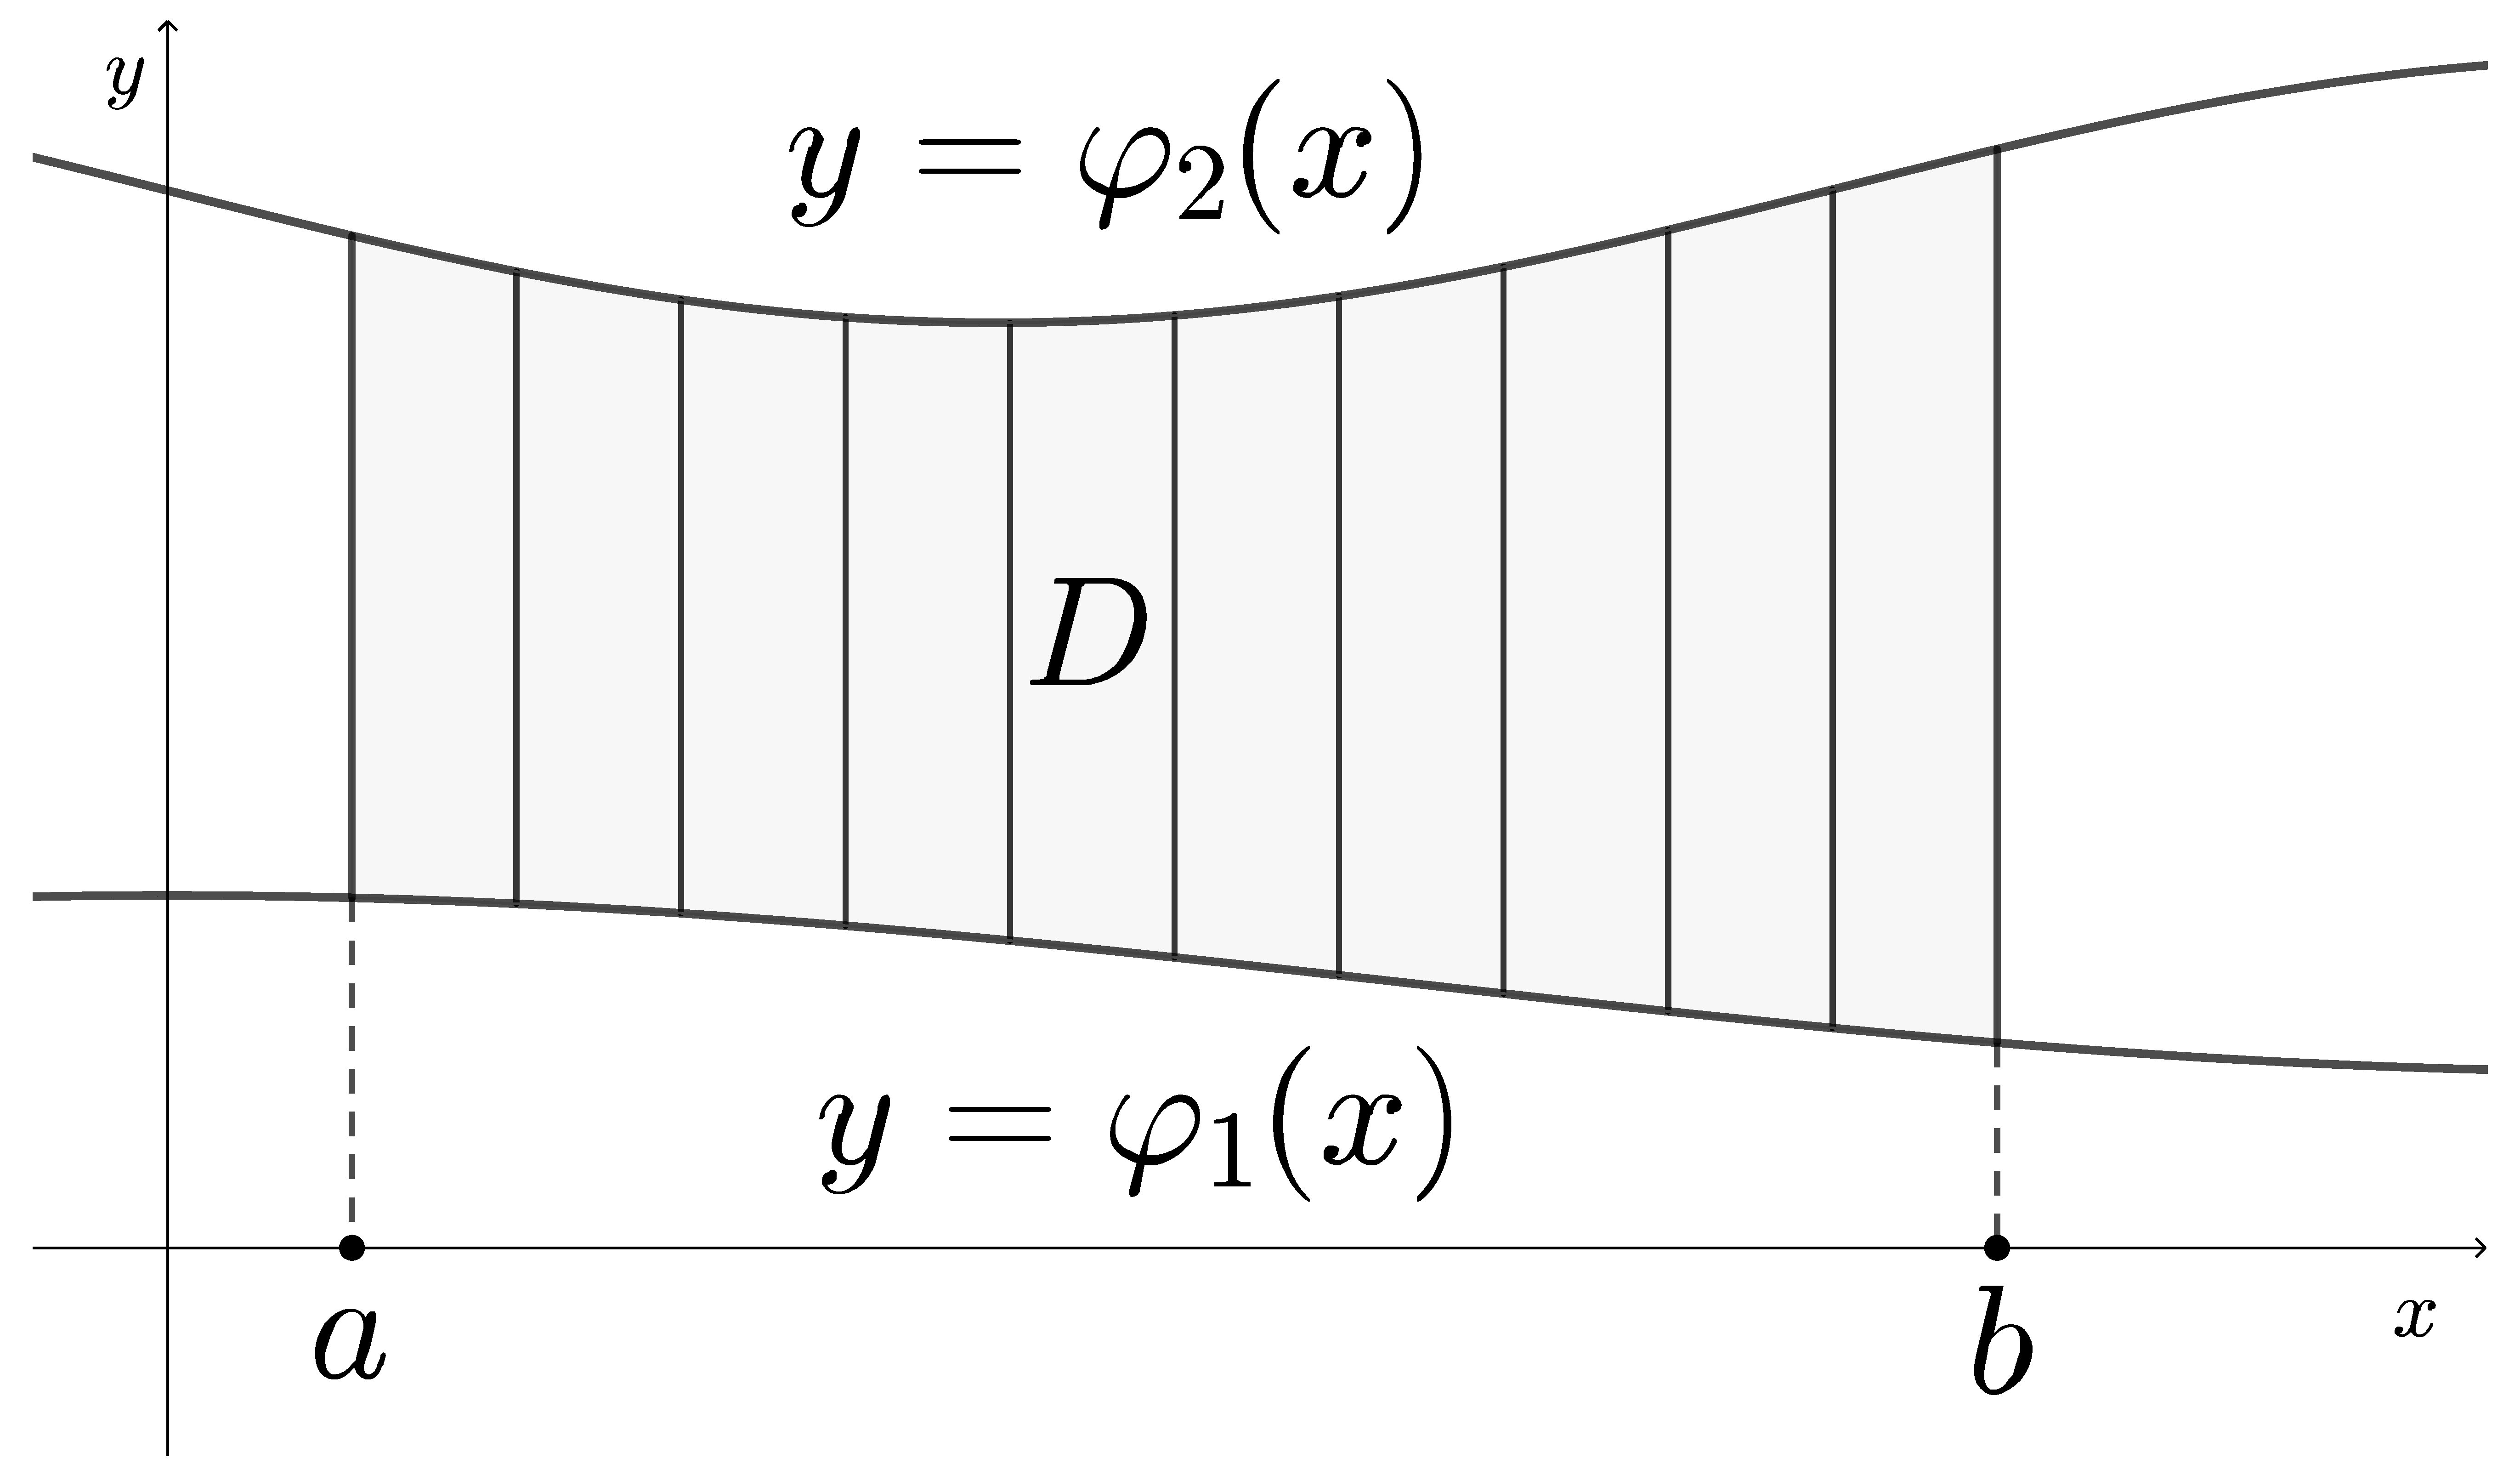
\includegraphics[height=3.5cm]{08/columnset.pdf}
    \end{minipage}
    \begin{minipage}{0.45\linewidth}
      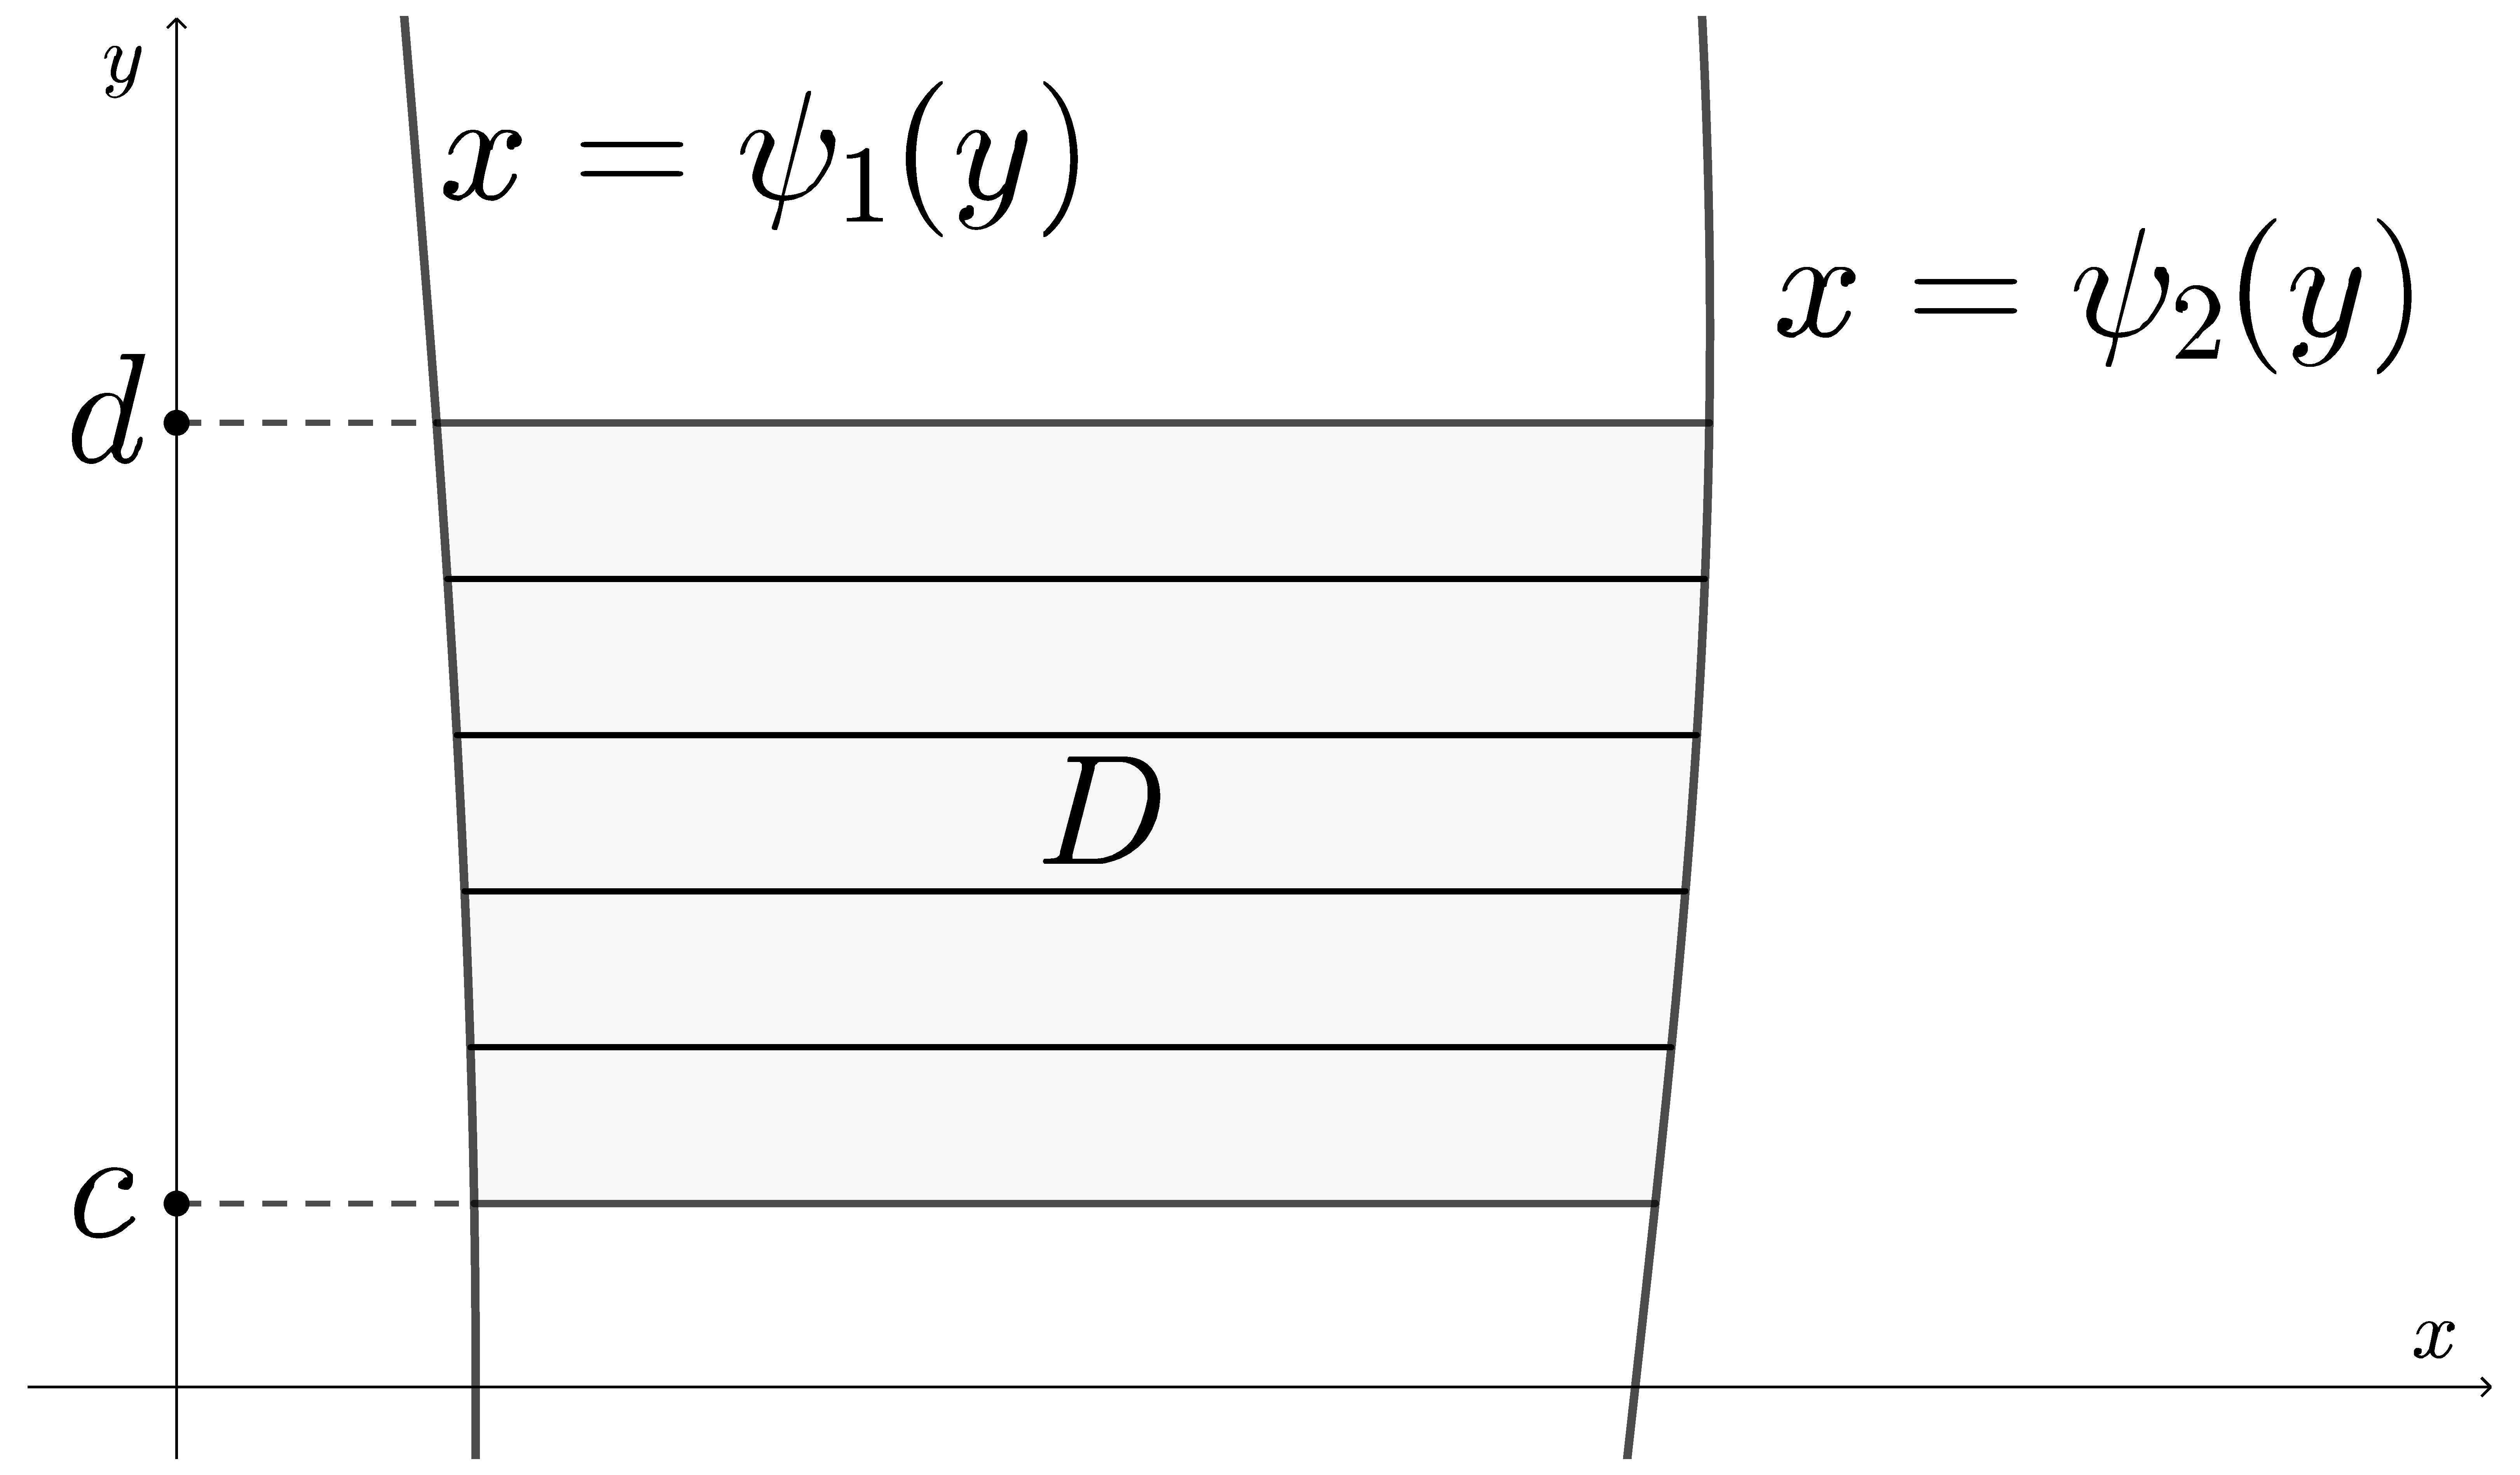
\includegraphics[height=3.5cm]{08/rowset.pdf}
    \end{minipage}
  \end{tabular}
\end{figure}

\begin{example}
  $D=\Set{(x,y) | 1 \leqq x \leqq 2, \, 0 \leqq y \leqq x}$
  に対して,$\ds \iint_{D}(x+y) \ dx dy$ は次のように計算できる.
  \begin{align*}
    \iint_{D} (x+y) \ dx dy 
    &= \int_{1}^{2} \left( \int_{0}^{x} (x+y) \ dy \right) dx
      = \int_{1}^{2} \left[ xy + \frac{1}{2}y^2 \right]_{y=0}^{y=x} dx\\
    &= \int_{1}^{2}\frac{3}{2} x^2 \ dx = \frac{1}{2}\Big[ x^3\Big]_{1}^{2} = \frac{7}{2}
  \end{align*}
\end{example}

\newpage

\subsection{定理\ref{thm:iterated2}の幾何学的意味}

$2$ 変数関数 $f(x,y)$ の有界閉領域 $D$ 上の2重積分は,$D$ の境界に
沿って伸びる $xy$ 平面に垂直な曲面と $xy$ 平面と $z=f(x,y)$ で囲まれる
立体の体積に等しい.ただし,$xy$ 平面よりも下側にある部分の体積は負の値
として扱う.定理\ref{thm:iterated2}の累次積分の内側に
\[
  F(x) = \int_{\phi_1(x}^{\phi_2(x)} f(x,y) \ dy, \quad
  G(y) = \int_{\psi_1(y)}^{\psi_2(y)} f(x,y) \ dx
\]
と名前を付ける.$F(\xi)$ の値は下図のように平面 $x=\xi$
によって立体を切ったときの断面積に等しい.同様に $G(\eta)$ の値は平
面 $y=\eta$ で立体を切ったときの断面積に等しい.従って,定
理\ref{thm:iterated2}は\textbf{立体の断面積を積分したものが体積である}こ
とを主張している.

\begin{figure}[h]
  \centering
  \includegraphics[height=11cm]{08/cutx.pdf}
\end{figure}


\newpage

\subsection{練習問題}

次の2重積分を求めよう.

\vspace{1zh}

\begin{enumerate}[(1)]

  \setlength{\itemsep}{2zh}

\item $\ds \iint_{D} \sin (x+y) \ dx dy, \quad D=\Set{(x,y) | 0 \leqq y \leqq \frac{\pi}{2}, \, 0 \leqq x \leqq y}$

\item $\ds \iint_{D} x \ dx dy, \quad D=\Set{(x,y) | y \leqq x \leqq \sqrt{y}}$
\item $\ds \iint_{D} xy \ dx  dy, \quad D=\Set{(x,y) | x+y \leqq 2, \, y^2 \leqq x, \, 0 \leqq y}$

\item $\ds \iint_{D} \sin\left( \pi x^2\right) \ dx dy, \quad D=\Set{(x,y) | y \leqq x \leqq 1, \, 0 \leqq y \leqq 1}$
  
\item $\ds \iint_{D} y \ dx dy, \quad D=\Set{(x,y) | \frac{y}{2} \leqq x \leqq 2y, \, x+y \leqq 1}$
  
\item $\ds \iint_{D} x \ dx dy, \quad D=\Set{(x,y) | -2 \leqq x \leqq 1, \, x^2+4x+1 \leqq y \leqq -x^2+2x+1}$
\end{enumerate}

\vspace{3zh}

「積分基本問題集 弍」(1) $\sim$ (4), (11), (14), (15) も参考にしてください.
\begin{center}
  \url{https://github.com/kazutsumi/Integral2/blob/main/integral2.pdf}
\end{center}

\begin{figure}[b]
  答え:(1) $1$ \quad (2) $\ds \frac{1}{12}$ \quad (3) $\ds \frac{3}{8}$ \quad
  (4) $\ds \frac{1}{\pi}$ \quad (5) $\ds \frac{1}{18}$ \quad (6) $\ds -\frac{1}{6}$
\end{figure}

\newpage

\subsection{(おまけ)定理\ref{thm:iterated2}の証明}\label{subsec:pf-iterated2}

定理\ref{thm:iterated2}の(1)を証明する.ただし,$f$ が $D$ 上で重積分可能
であることの証明は省略する.\\


1変数関数の積分に関する以下の定理\ref{thm:piecewise}を使う.

\begin{theorem}\label{thm:piecewise}
  有界閉区間で区分的に連続な $1$ 変数関数はこの区間で積分可能である.
\end{theorem}

有界閉区間 $[a,b]$ で定義された $1$ 変数関数
$f$が有限個の点$c_1, c_2, \ldots, c_n \in [a,b]$ を除いて連続で,
各 $c_i$における左側極限 $\ds \lim_{x \to c_i-0} f(x)$ と
右側極限$\ds \lim_{x \to c_i+0} f(x)$ が存在すると
き,$f(x)$ は $[a,b]$ で\textbf{区分的に連続}であるという.ただし,両
端 $a,b$では区間の内側からの片側極限のみ存在すればよい.すなわち,$a$
では右側極限が,$b$ では左側極限のみが存在すればよい.区分的に連続な関
数は有界である.また,連続関数は区分的に連続である.
\begin{figure}[h]
  \centering
  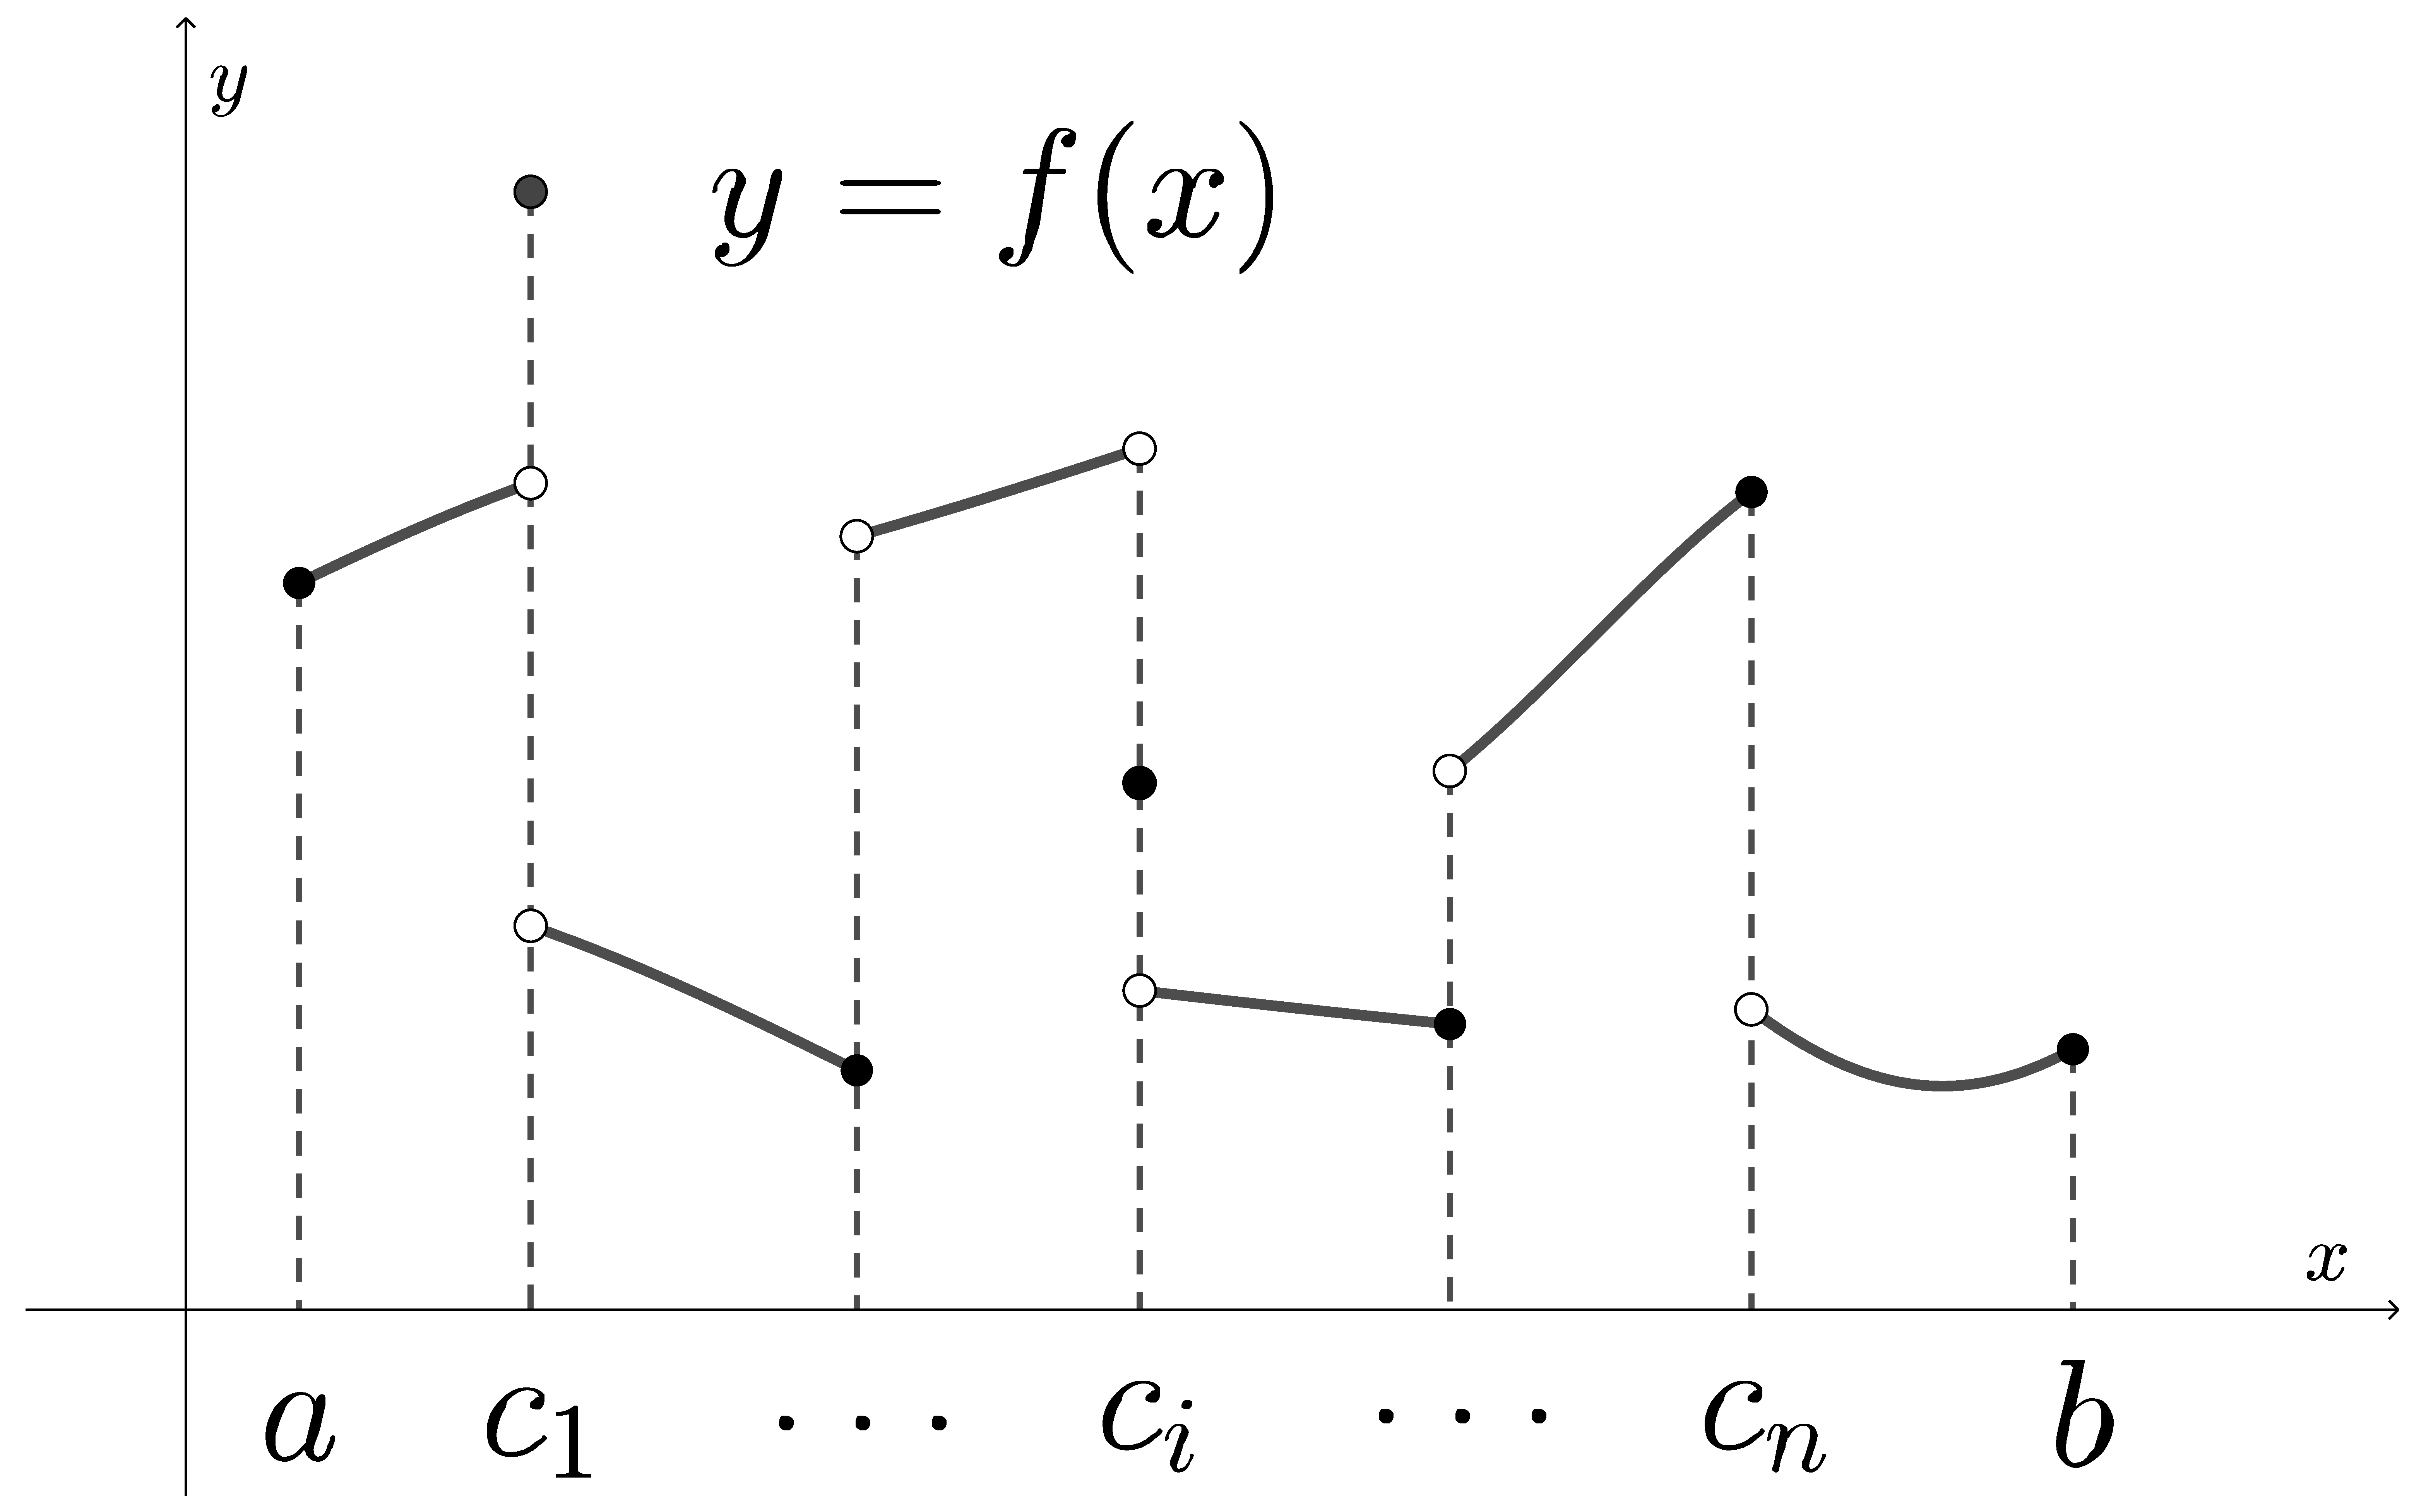
\includegraphics[height=6cm]{08/piecewise.pdf}
\end{figure}

有界閉区間 $[a,b]$ で区分的に連続な関数 $f$ の積分は,区分ごとの積分値
を足し合わせればよい.つまり,不連続な点
$c_1, c_2, \ldots, c_n \in [a,b] \; (c_1 < c_2 < \cdots <
c_n)$ と $c_0=a, \; c_{n+1}=b$ に対し
\[
  f_i(x) = \left\{
  \begin{array}{cl}
    \ds \lim_{x \to c_{i-1}+0} f(x) & (x=c_{i-1})\\
    f(x) & (c_{i-1} < x < c_{i})\\
    \ds \lim_{x \to c_{i}-0} f(x) & (x=c_{i})
  \end{array}
  \right. , \; i=,1, \ldots, n+1
\]
とすれば,各 $f_i$ は $[c_{i-1},c_{i}]$ で連続なので以下が成り立つ.
\[
  \int_{a}^{b} f(x) \ dx = \sum_{i=1}^{n+1} \int_{c_{i-1}}^{c_{i}} f_i(x) \ dx
\]


\newpage


\begin{proof}[\textbf{定理\ref{thm:iterated2}(1)の証明}]

  下図のように $D$ を含む長方形 $K=[a,b] \times [c,d]$ をとる.
    \begin{figure}[h]
    \centering
    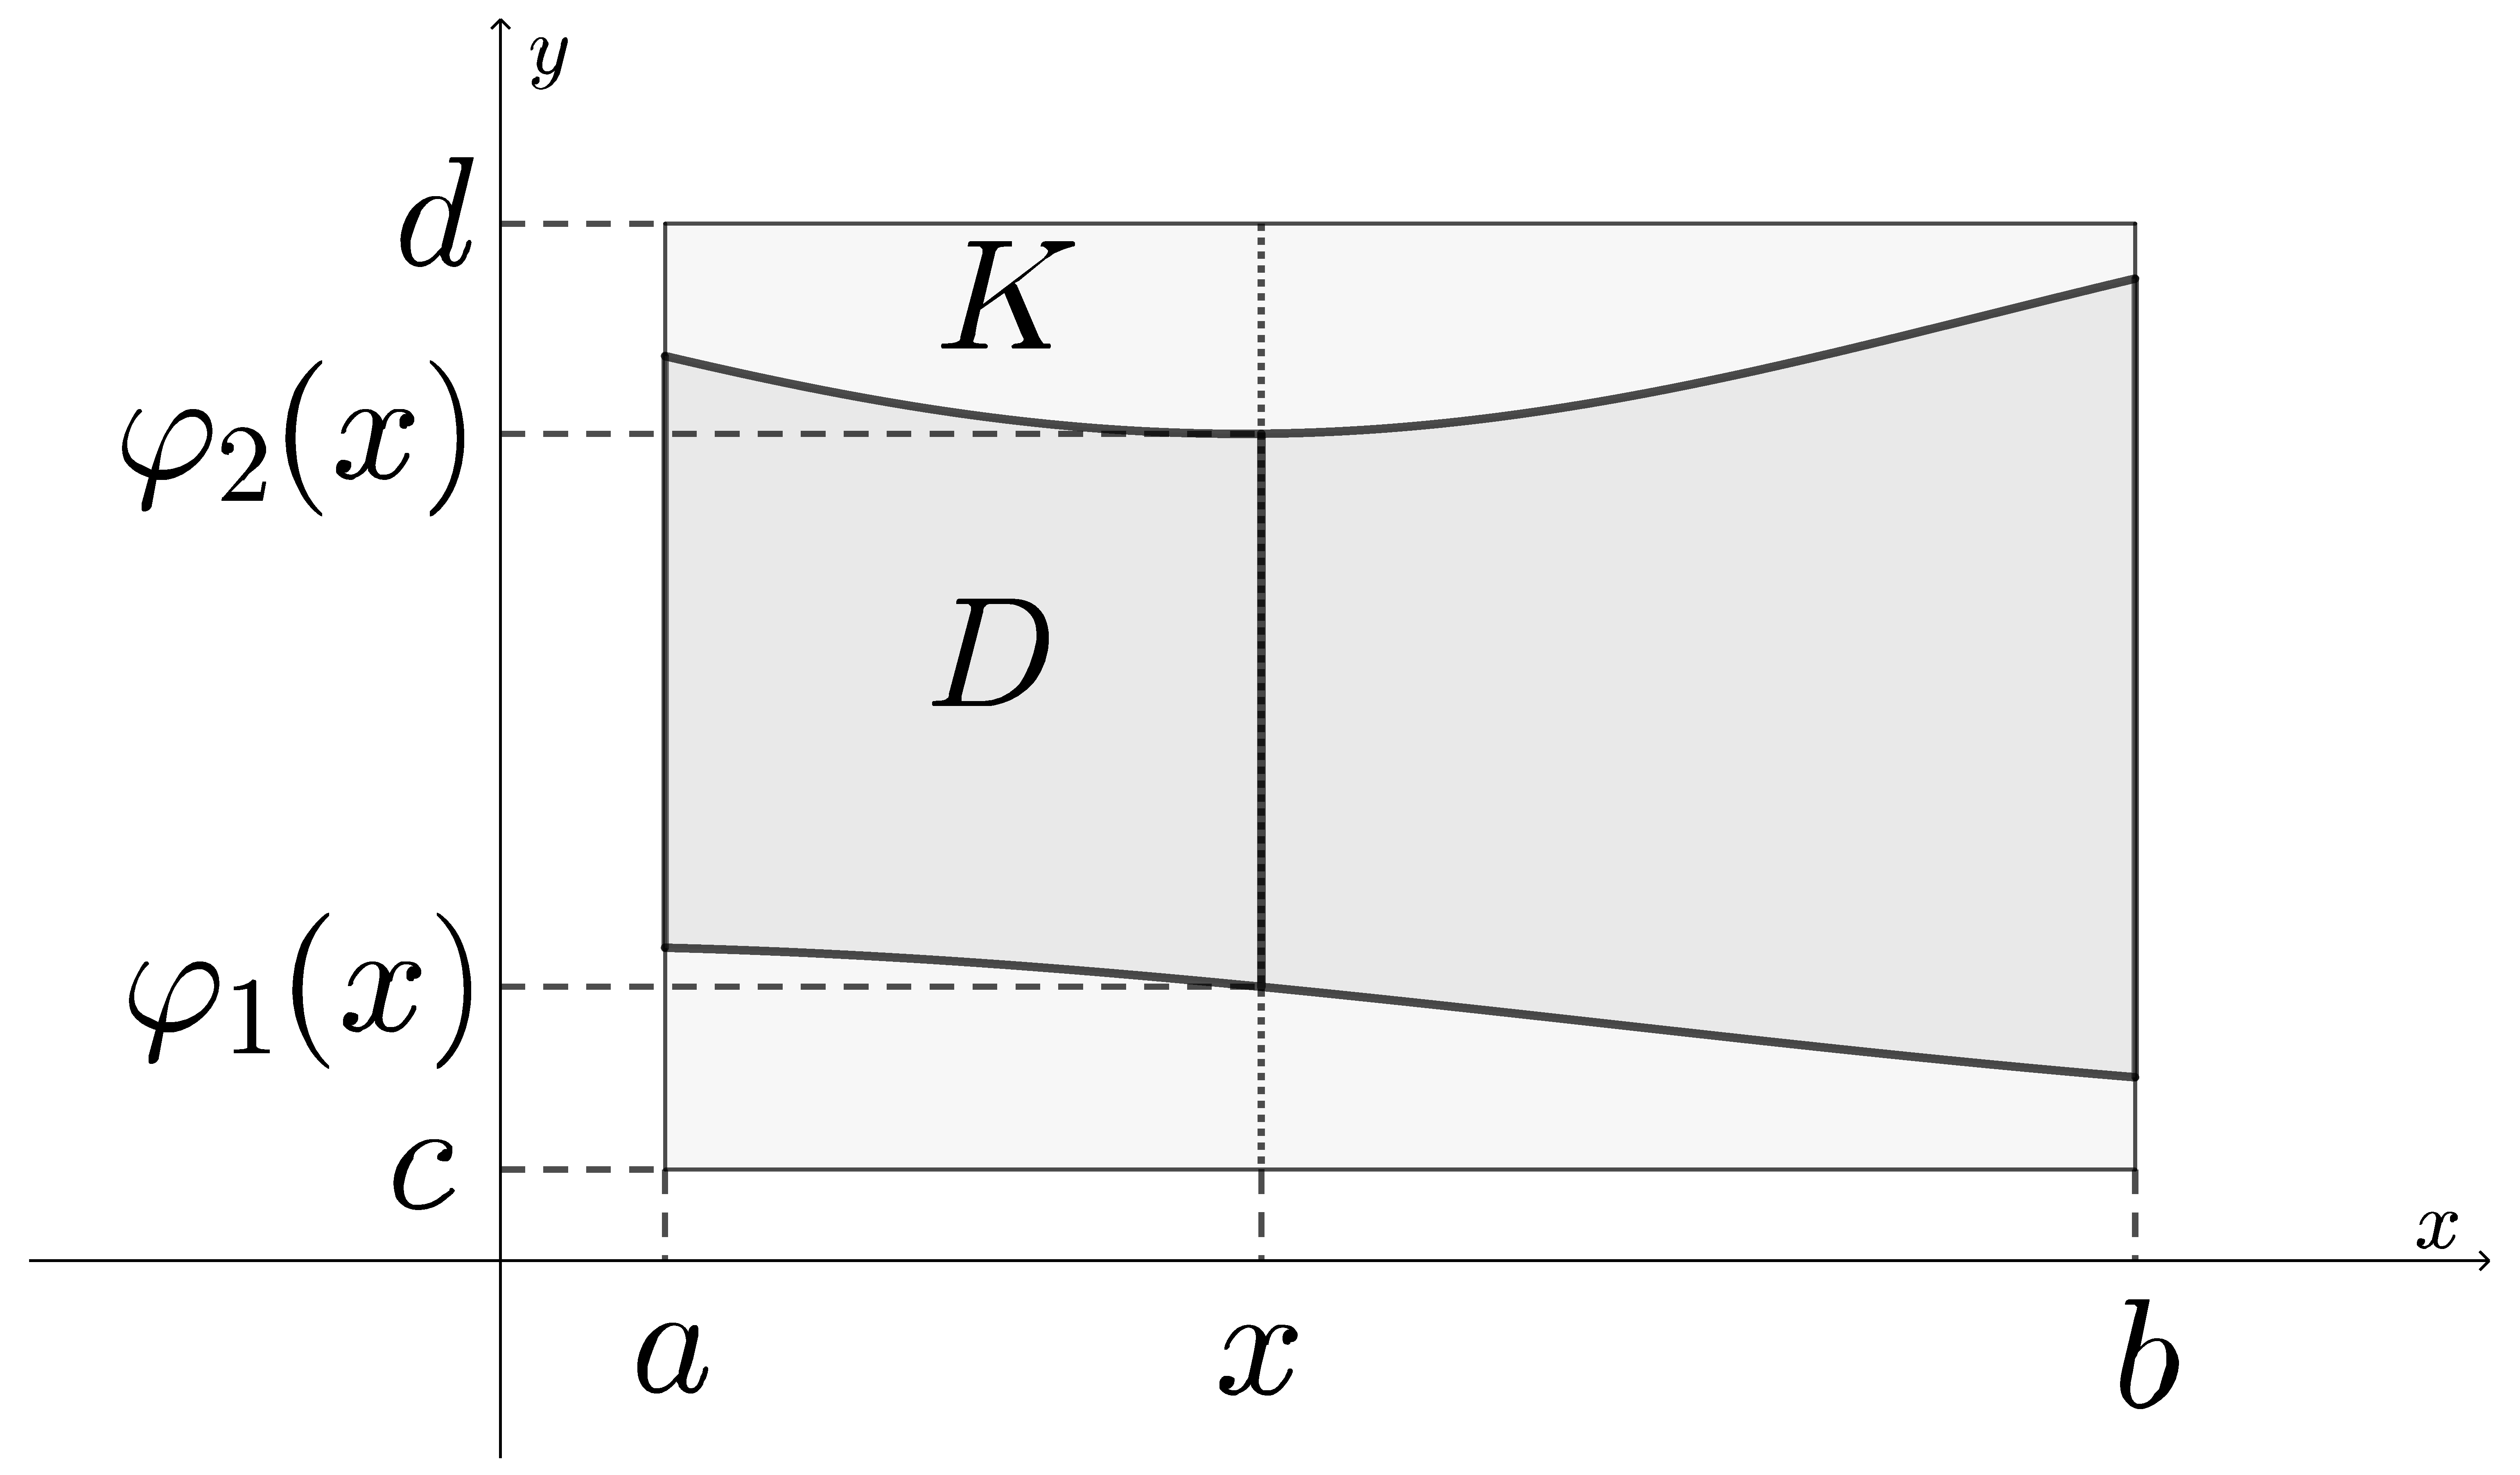
\includegraphics[height=5cm]{08/columnK.pdf}
  \end{figure}

  \noindent ここで $K$ 上の関数 $f^*$ を
  \[
    f^*(x,y) = \left\{
    \begin{array}{cl}
      f(x,y) & \left( (x,y) \in D\right)\\
      0 & \left( (x,y) \notin D \right)
    \end{array}
    \right.
  \]
  により定める.$f$ は $D$ 上重積分可能(証明略)だから,有界閉領域上
  の2重積分の定義から $f^*$ は $K$ 上重積分可能で,
  \begin{equation}\label{eq:D-K}
    \iint_{D} f(x,y) \ dx dy = \iint_{K} f^{*}(x,y) \ dx dy
  \end{equation}
  である.任意の $\xi \in [a,b]$ に対して,$y$ の $1$ 変数関
  数 $f^{*}(\xi , y)$ は $[c,d]$ において
  $\varphi_1(\xi), \varphi_2(\xi)$ を不連続点とする区分的に連続な関数であ
  る.従って,定理\ref{thm:piecewise}より $f^{*}(\xi,y)$ は$[c,d]$ で積
  分可能で,
  \begin{align*}
    \int_{c}^{d} f^{*}(\xi,y) \ dy 
    &= \int_{c}^{\varphi_1(\xi)} f^{*}(\xi, y) \ dy + \int_{\varphi_1(\xi)}^{\varphi_2(\xi)} f^{*}(\xi, y) \ dy 
      + \int_{\varphi_2(\xi)}^{d} f^{*}(\xi,y) \ dy\\
    &= 0 + \int_{\varphi_1(\xi)}^{\varphi_2(\xi)} f^{*}(\xi, y) \ dy  +0
      = \int_{\varphi_1(\xi)}^{\varphi_2(\xi)}f(\xi ,y) \ dy
  \end{align*}
  である.従って,$1$ 変数関数 $\ds F(x) = \int_{c}^{d}f^{*}(x, y) \
  dy$ が $[a,b]$ で積分可能で,かつ以下が成り立つことを証明すればよい.
  \[
    \iint_{K} f^{*}(x,y) \ dx dy = \int_{a}^{b} \left( \int_{c}^{d} f^{*}(x,y) \ dy\right) dx
  \]
  
  $\Delta=(x_0, \ldots, x_m;\ y_0, \ldots, y_n)$
  を長方形$K=[a,b] \times [c,d]$ の任意の分割とする.$x$ 方向の各小区
  間 $[x_{i-1},x_{i}]$ から代表点 $\xi_i$ を任意に選ぶ.$y$ 方向の各小
  区間 $[y_{j-1}, y_{j}]$ での $f^{*}(\xi_i, y)$ の最小値
  を $m_{ij}=f^{*}(\xi_i, s_{ij})$ とし,最大値を$M_{ij}=f^{*}(\xi_i,
  S_{ij})$ とすると,各小区間 $[y_{j-1},y_{j}]$ で
  $m_{ij} \leqq f^{*}(\xi_i, y) \leqq M_{ij}$ だから,
  \[
    m_{ij}(y_{j}-y_{j-1}) \leqq \int_{y_{j-1}}^{y_j} f^{*}(\xi_i, y) \ dy \leqq M_{ij} (y_{j} - y_{j-1})
  \]
  である.これが各 $i, j$ で成り立つので以下の不等式が成り立つ.
  \begin{align*}
    \sum_{i=1}^{m} \sum_{j=1}^{n} m_{ij} (x_{i}-x_{i-1})(y_{j}-y_{j-1})
    & \leqq \sum_{i=1}^{m}\left( \sum_{j=1}^{n} \int_{y_{j-1}}^{y_j}f^{*}(\xi_i,y) \ dy \right)(x_{i}-x_{i-1})\\
    & \leqq \sum_{i=1}^{m} \sum_{j=1}^{n} M_{ij} (x_{i}-x_{i-1})(y_{j}-y_{j-1})
  \end{align*}
  この不等式の左辺は$\Delta$ と $\Set{\left(\xi_i, s_{ij}\right)}$ に関
  する $f^{*}$ の Riemann 和であり,右辺
  は $\Delta$ と $\Set{\left(\xi_i, S_{ij} \right)}$ に関する $f^{*}$
  の Riemann 和である.また,不等式の中辺は
  \begin{align*}
    \sum_{i=1}^{m} \left( \sum_{j=1}^{n} \int_{y_{j-1}}^{y_j} f^{*}(\xi_i, y) \ dy \right) (x_i-x_{i-1})
   & =\sum_{i=1}^{m} \left( \int_{c}^{d} f^{*}(\xi_i, y) \ dy\right) (x_{i}-x_{i-1})\\
   & = \sum_{i=1}^{m} F(\xi_i)(x_{i}-x_{i-1})
  \end{align*}
  である.これは区間 $[a,b]$ の分割 $\Delta_X=(x_0, \ldots, x_m)$ と代
  表点集合 $\Set{\xi_i}$ に関する $1$ 変数関数 $F$ の Riemann 和である.
  よって,以下の不等式が成り立つ.
  \[
    R\left( \Delta, \Set{\left(\xi_i, s_{ij}\right)}, f^{*}\right) \leqq R\left(\Delta_{X},\Set{\xi_i}, F\right)
    \leqq R\left( \Delta, \Set{\left(\xi_i, S_{ij}\right)}, f^{*}\right)
  \]
  $f^{*}$ は $K$ 上重積分可能なので,$|\Delta| \to 0$ のときこ
  の不等式の左辺と右辺,従って中辺も,(\ref{eq:D-K})に収束する.ま
  た,$|\Delta| \to 0$ のとき $|\Delta_X| \to 0$ であるか
  ら,$F$ は $[a,b]$ で積分可能であり,以下を得る.
  \[
    \begin{aligned}
    \iint_{K}f^{*}(x,y) \ dx dy 
    &= \lim_{|\Delta| \to 0} R\left( \Delta, \Set{\left(\xi_i, s_{ij}\right)}, f^{*}\right)
    = \lim_{|\Delta| \to 0} R\left( \Delta, \Set{\left(\xi_i, S_{ij}\right)}, f^{*}\right)\\
    &= \lim_{|\Delta_X| \to 0} R\left( \Delta_X, \Set{\xi_i}, F\right)\
    = \int_{a}^{b} F(x) \ dx \\
    &= \int_{a}^{b} \left( \int_{c}^{d} f^{*}(x,y) \ dy \right) dx
  \end{aligned}
\]
\end{proof}



\end{document}
